\documentclass{beamer}

\usetheme{Madrid}

\usepackage{graphicx}
\usepackage{booktabs}

\title{Intrusion Detection on UNSW-NB15}
\subtitle{Binary and Multiclass Classification of Network Traffic}
\author{Simone Montagnini}
\institute{University of Bologna}
\date{September 2026}

\begin{document}

\frame{\titlepage}

\begin{frame}{Outline}
  \tableofcontents
\end{frame}

\section{Introduction}

\begin{frame}{Project Objectives}
  This project addresses intrusion detection on network traffic through two
  classification tasks:
  \begin{itemize}
    \item \textbf{Binary classification}: distinction between normal and malicious traffic
      (\texttt{label})
    \item \textbf{Multiclass classification}: identification of the specific threat among 9 possible types
      (\texttt{attack\_cat})
  \end{itemize}
  \vspace{0.5cm}
  \begin{block}{Source}
  Kaggle competition: \href{https://www.kaggle.com/competitions/advanced-ai-for-cybersecurity-intrusion-detection-with-unsw-nb-15/overview}{\textit{Advanced AI for Cybersecurity — Intrusion Detection with UNSW-NB15}}
  \end{block}
\end{frame}

\begin{frame}{The Dataset — UNSW-NB15}
  \begin{itemize}
    \item Realistic network traffic dataset with both normal and
      malicious network activity
    \item \textbf{175,341} training records, \textbf{42} original features
      (categorical and numerical)
    \item Two target columns:
      \begin{itemize}
        \item \texttt{label}: 0 = normal, 1 = attack
        \item \texttt{attack\_cat}: Normal, Generic, Exploits, Fuzzers, DoS,
          Reconnaissance, Analysis, Backdoor, Shellcode, Worms
      \end{itemize}
  \end{itemize}
\end{frame}

\section{Exploratory Data Analysis}

\begin{frame}{Target Distribution}
  \begin{columns}
    \column{0.5\textwidth}
    \textbf{Binary (\texttt{label})}
    \begin{itemize}
      \item Attack: 68.1\%
      \item Normal: 31.9\%
    \end{itemize}

    \column{0.5\textwidth}
    \textbf{Multiclass (\texttt{attack\_cat})}
    \begin{itemize}
      \footnotesize
      \item Normal: 56,000
      \item Generic: 40,000
      \item Exploits: 33,393
      \item Fuzzers: 18,184
      \item DoS: 12,264
      \item Reconnaissance: 10,491
      \item Analysis: 2,000
      \item Backdoor: 1,746
      \item Shellcode: 1,133
      \item \textbf{Worms: 130}
    \end{itemize}
  \end{columns}
  \vspace{0.3cm}
  \begin{alertblock}{Balancing}
    The binary target is reasonably balanced, but \texttt{attack\_cat} is
    severely imbalanced: Worms has $430\times$ fewer examples than Normal —
    need for \textbf{class-weighting} strategies in the multiclass model.
  \end{alertblock}
\end{frame}

\begin{frame}{Data Quality}
  \begin{itemize}
    \item \textbf{Duplicate rows}: 78,519 out of 175,341 (\textbf{44.8\%})
      \begin{itemize}
        \item Removed before splitting, to avoid data leakage between
          train and test
      \end{itemize}
    \vspace{0.3cm}
    \item \textbf{Categorical features profile}:
      \begin{itemize}
        \item \texttt{proto} (High cardinality): 133 unique values (\texttt{tcp}/\texttt{udp}
          $\approx$ 82\% of traffic)
        \item \texttt{service}: 13 values, 54\% missing/unknown (\texttt{-})
        \item \texttt{state}: 9 values
      \end{itemize}
  \end{itemize}
\end{frame}

\begin{frame}{Skewed Numerical Features}
  Several traffic features show extreme right-skewed distributions:
  \begin{center}
    \begin{tabular}{lr}
      \toprule
      \textbf{Feature} & \textbf{Skewness} \\
      \midrule
      trans\_depth & 167.3 \\
      response\_body\_len & 76.3 \\
      sbytes & 45.3 \\
      sloss & 44.8 \\
      dloss & 41.4 \\
      spkts & 40.2 \\
      \bottomrule
    \end{tabular}
  \end{center}
  \vspace{0.3cm}
  \textbf{27 features} exceeded the skewness threshold ($> 1.0$) and were logarithmic transformed (\texttt{log1p}) in preprocessing.
\end{frame}

\section{Preprocessing}

\begin{frame}{Data Preparation \& Transformation}
  \begin{enumerate}
    \item \textbf{Duplicate removal}: removed 78,519 duplicate rows before
      splitting
    \item \textbf{Train/test split}: 67/33, stratified on \texttt{label}
    \item \textbf{Encoding}: \texttt{OneHotEncoder} on \texttt{proto},
      \texttt{service}, \texttt{state} — 185 total features
    \item \textbf{Skewness correction}: \texttt{log1p} transform on 27
      features (skewness $> 1.0$)
  \end{enumerate}
\end{frame}

\begin{frame}{Avoiding Data Leakage}
  \begin{alertblock}{Key methodological choice}
    Preprocessing steps are \textbf{fit exclusively on the training set} and mapped to the test set via \texttt{transform()} in order to prevent data leakage.
  \end{alertblock}
  \vspace{0.3cm}
  \begin{itemize}
    \item \textbf{Strict separation}: Fitting encoders on the entire dataset injects future knowledge into the training phase
    \item \textbf{Handling unseen data}: Rare categories (e.g. within the 133 \texttt{proto} values) might appear exclusively in the test set
    \item \textbf{Fault tolerance}: \texttt{OneHotEncoder} is configured 
      with \texttt{handle\_unknown='ignore'} to safely bypass novel 
      categories without causing execution failures
  \end{itemize}
\end{frame}

\section{Attribute Selection}

\begin{frame}{SelectKBest}
  \begin{itemize}
    \item \textbf{Supervised feature selection}: each feature is scored against the
      target, keeping only the top $k$ features
\item \textbf{Score function}: ANOVA F-value (\texttt{f\_classif})
      \begin{itemize}
        \item \texttt{mutual\_info\_classif} was excluded due to extreme
          computation times on this dataset's dimensionality.
      \end{itemize}
    \item \textbf{Selection}: $k = 50$ out of 185 features, selected separately for the
      \texttt{label} and \texttt{attack\_cat} targets
  \end{itemize}
  \vspace{0.3cm}
  \begin{block}{Interpretability Preservation}
    SelectKBest retains the original traffic attributes. This ensures the model remains transparent, enabling direct attribution of malicious activity to specific network signals.
  \end{block}
\end{frame}

\begin{frame}{PCA}
  \begin{itemize}
    \item \textbf{Prerequisite scaling}: features standardized (\texttt{StandardScaler}), then PCA fitted
      on the training set only
    \item \textbf{Explained variance}: retaining 90\% of the variance requires \textbf{137 components} (118 for 80\%) 
    \item \textbf{Limited reduction}: 137 components out of 185 features
  \end{itemize}
  \vspace{0.3cm}
  \begin{block}{Component Analysis \& Feature Contribution}
    Rather than being dominated by the numerous one-hot encoded columns \texttt{proto}, the principal components exhibit a mix of underlying data types. For instance, PC2 is driven almost entirely by timing and byte-related numerical features (\texttt{sinpkt}, \texttt{dload}, \texttt{tcprtt})
  \end{block}
\end{frame}

\begin{frame}{Feature Selection Comparison}
    \small
    \begin{tabular}{lcc}
      \toprule
       & \textbf{SelectKBest} & \textbf{PCA} \\
      \midrule
      Dimensionality & 50 features & 137 components \\
      Interpretability & High (original domain) & Low (linear combinations) \\
      Transformation & Supervised (target-aware) & Unsupervised \\
      Training efficiency & Acceptable & Impractical \\
      \bottomrule
    \end{tabular}
  \vspace{0.3cm}
  \begin{alertblock}{Design Choice}
    PCA was excluded from the classification pipeline: even with a reduced number of
    components, the computational overhead during GridSearchCV was impractical. Classification
    proceeds with SelectKBest only.
  \end{alertblock}
\end{frame}

\section{Classification}

\begin{frame}{Classification Methodology}
  \begin{itemize}
    \item \textbf{Algorithms}: Decision Tree (as a baseline) and Random Forest
    \item \textbf{Hyperparameter Tuning}: \texttt{max\_depth} and \texttt{criterion} for Decision Tree, \texttt{n\_estimators} and \texttt{max\_depth} for Random Forest, \texttt{class\_weight} \texttt{None} vs \texttt{'balanced'} for both
    \item \textbf{Imbalance Handling}: Included \texttt{class\_weight} (\texttt{None} vs \texttt{'balanced'}) to evaluate the best strategy for rare threat vectors
    \item \textbf{Validation}: 5-fold \texttt{StratifiedKFold} to ensure 
      proportional representation of all classes during training
  \end{itemize}
  \vspace{0.2cm}
  \begin{block}{Evaluation Metrics}
    Accuracy is misleading on highly imbalanced datasets. Models are evaluated 
    using \textbf{F1-Score} (Binary classification) and \textbf{Macro F1-Score} 
    (Multiclass classification) to weigh the performance on minority classes equally.
  \end{block}
\end{frame}

\begin{frame}{Binary Classification Results}
  \begin{columns}
    \column{0.5\textwidth}
    \hspace{1.1cm}\textbf{Model Performance} \\
    \vspace{0.2cm}
    \small
    \hspace{0.5cm}
    \begin{tabular}{lcc}
      \toprule
      \textbf{Metric} & \textbf{DT} & \textbf{RF} \\
      \midrule
      Accuracy & 0.916 & 0.920 \\
      Precision & 0.918 & 0.923 \\
      Recall & 0.916 & 0.920 \\
      \textbf{F1-Score} & \textbf{0.916} & \textbf{0.920} \\
      \bottomrule
    \end{tabular}

    \vspace{0.1cm}
    \hspace{0.8cm}{\tiny DT = Decision Tree, RF = Random Forest}
    
    \vspace{0.4cm}
    \begin{itemize}
      \item Random Forest achieves an excellent F1-Score of \textbf{0.920}.
      \item The model is \textbf{highly reliable} in distinguishing malicious 
      activity from normal traffic.
    \end{itemize}

    \column{0.5\textwidth}
    \begin{figure}
      \centering
      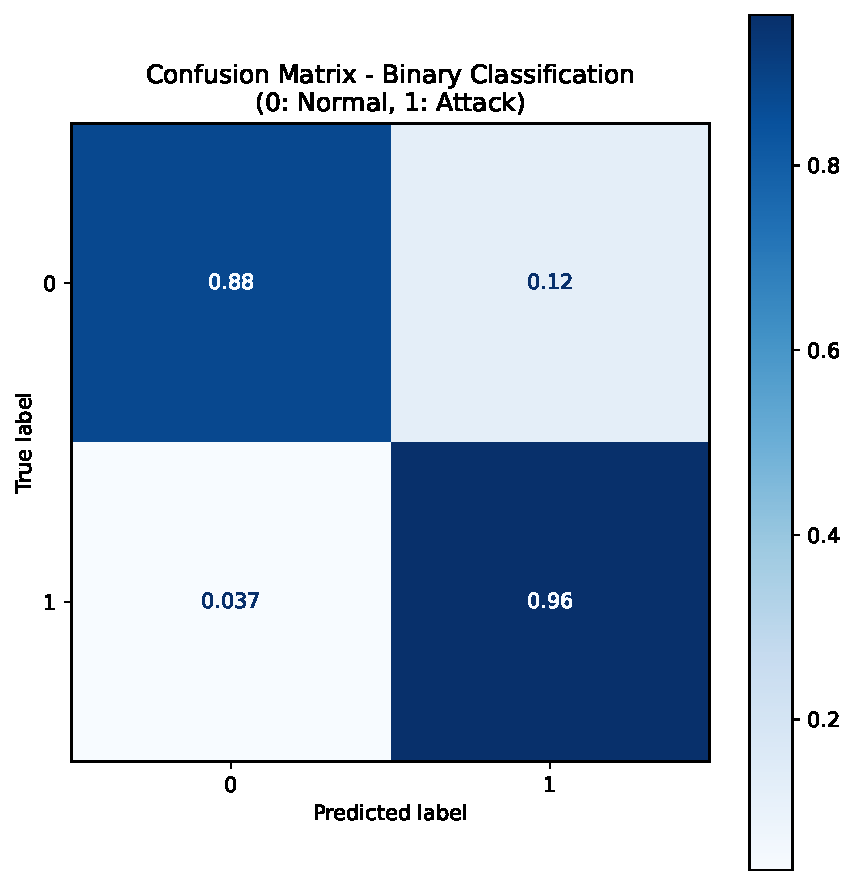
\includegraphics[height=0.65\textheight]{images/cm_binary.pdf}
      \caption{Binary Confusion Matrix}
    \end{figure}
  \end{columns}
\end{frame}

\begin{frame}{Multiclass Classification Results}
  \begin{columns}
    \column{0.55\textwidth}
    \textbf{The Multiclass Challenge} \\
    \vspace{0.2cm}
    \begin{itemize}
      \item Best model achieves a \textbf{Macro F1-Score} of \textbf{0.57}
      \item \textbf{Majority classes} (Normal, Generic) are predicted with 
        high confidence
      \item \textbf{Minority classes} drag the macro average down due to 
        overlapping feature spaces and extreme sparsity
    \end{itemize}
    \vspace{0.2cm}
    \begin{alertblock}{Impact of Balancing}
      Thanks to \texttt{class\_weight='balanced'}, the model 
      is also able to detect instances of ultra-rare attacks 
      (like Worms), preventing them from being completely ignored.
    \end{alertblock}

    \column{0.45\textwidth}
    \begin{figure}
      \centering
      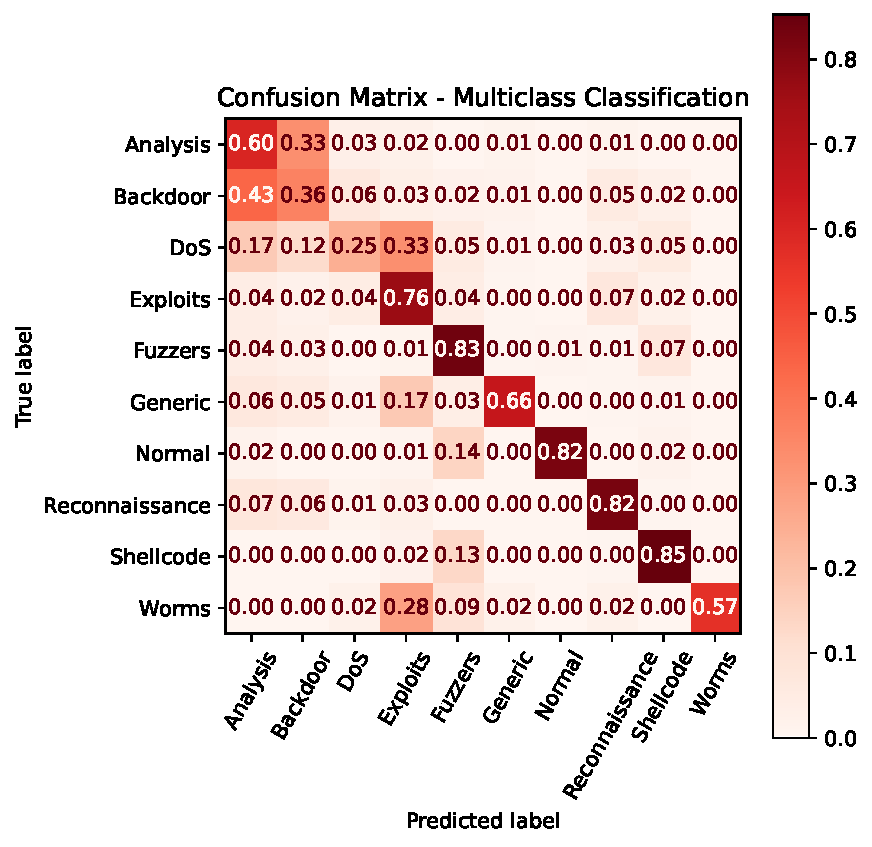
\includegraphics[width=\textwidth]{images/cm_multiclass.pdf}
      \caption{Multiclass Confusion Matrix}
    \end{figure}
  \end{columns}
\end{frame}

\begin{frame}{Feature Importance Analysis}
  \begin{itemize}
    \item \textbf{Binary task}: Mostly relies on TCP handshake timing features (\texttt{ackdat}, \texttt{synack}, \texttt{tcprtt}), anomalous handshakes are a strong indicator of malicious traffic
    \item \textbf{Multiclass task}: Based on byte-transfer volume features (\texttt{sbytes}, \texttt{smean}, \texttt{dbytes}) to differentiate the \textit{type} of attack 
  \end{itemize}

  \vspace{0.3cm}
  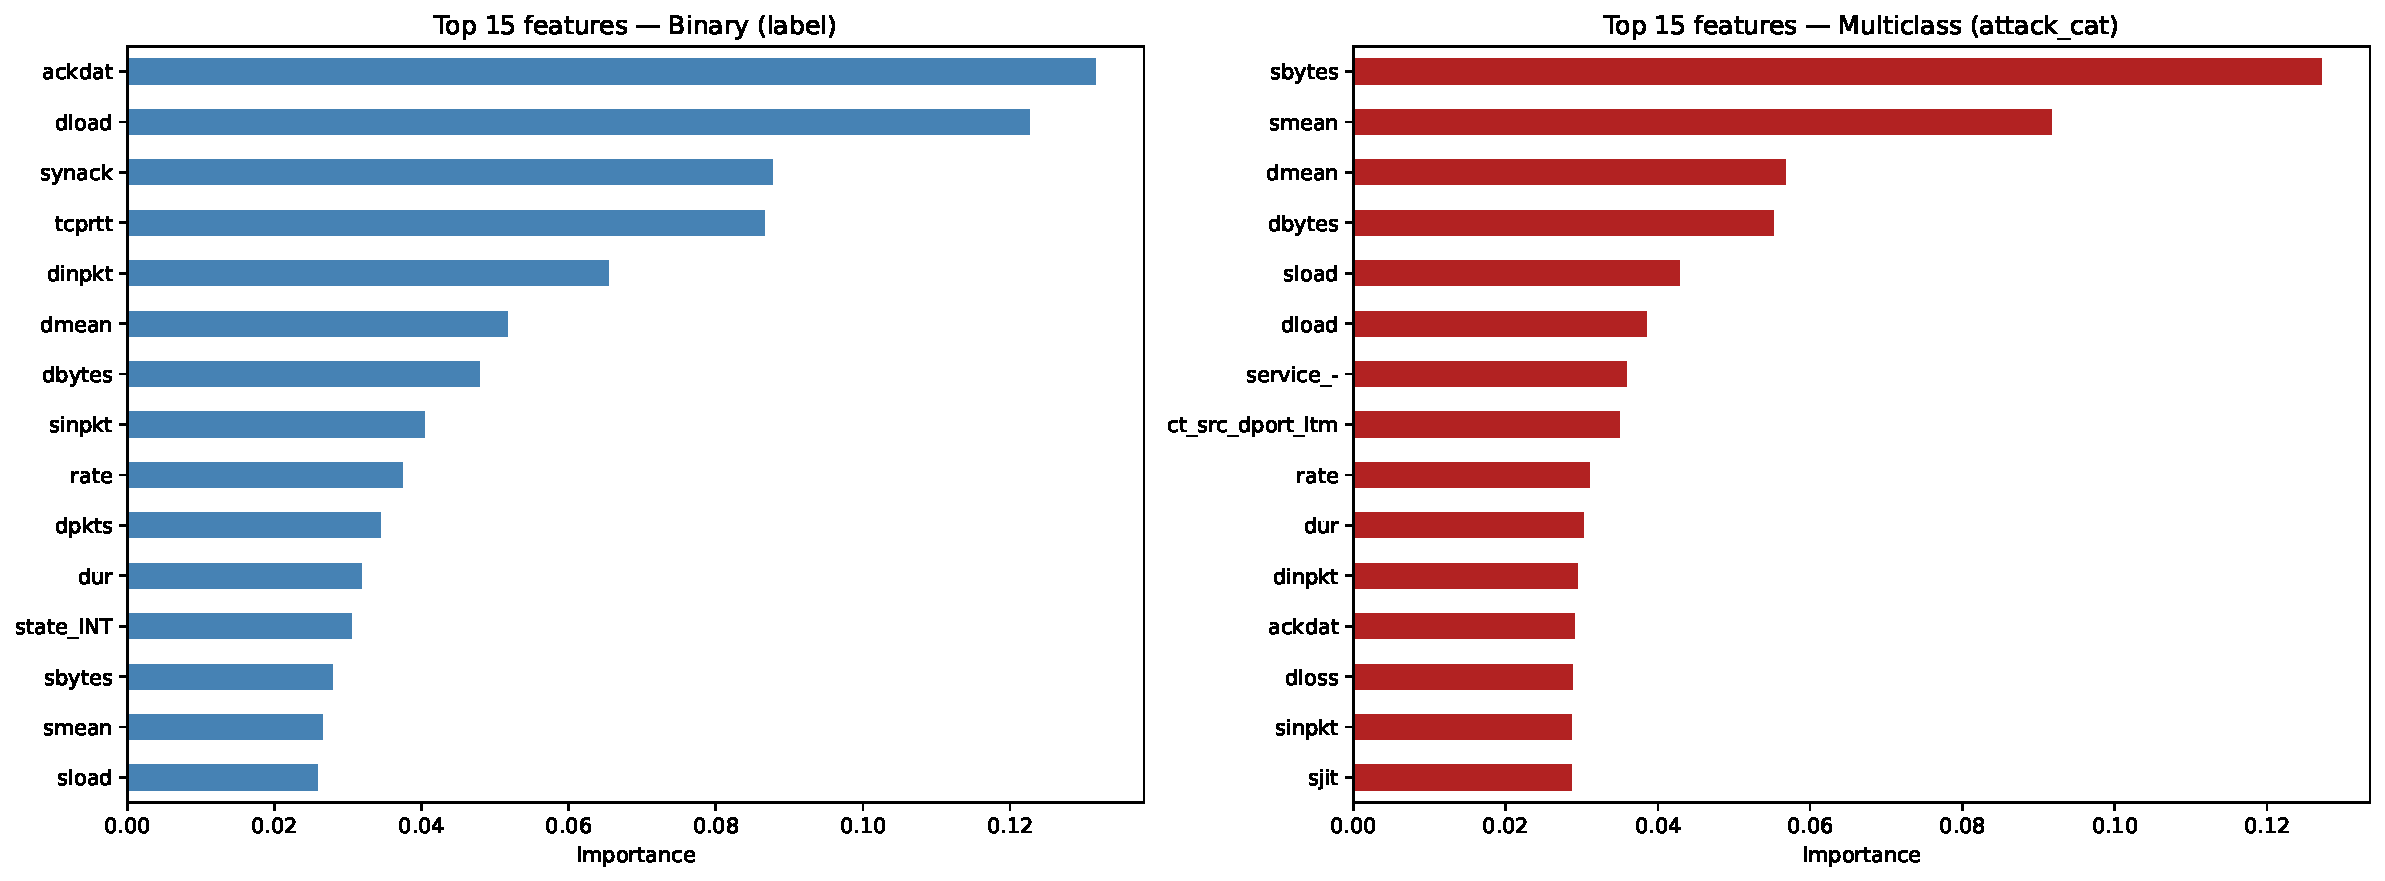
\includegraphics[width=\textwidth, height=0.55\textheight, keepaspectratio]{images/feature_importance.pdf}
\end{frame}

\section{Conclusions}

\begin{frame}{Project Evaluation}
  \begin{itemize}
    \item \textbf{Methodological trade-offs}: Prioritizing interpretability 
      (SelectKBest and Tree-based models) proved highly effective for binary 
      detection, achieving an F1-Score of 0.92 while maintaining transparent 
      decision rules
    \vspace{0.2cm}
    \item \textbf{The Multiclass bottleneck}: Differentiating specific attack 
      vectors remains intrinsically difficult (Macro F1: 0.57). The confusion matrix revealed concentrated overlap between related categories (e.g. DoS/Exploits, Backdoor/Analysis) and, notably, between Fuzzers and Normal traffic, independent of class imbalance
    \vspace{0.2cm}
    \item \textbf{Data Quality Dependency}: The project highlighted how extreme class 
      imbalance heavily constrain the theoretical upper bound of any 
      standard classifier's performance
  \end{itemize}
\end{frame}

\begin{frame}{Future Directions}
  To overcome the current limitations and push the system toward a realistic Network Intrusion Detection System, future iterations 
  could explore:
  
  \vspace{0.3cm}
  \begin{itemize}
    \item \textbf{Advanced Resampling}: Although SMOTE was initially considered, it was discarded due to extreme computational overhead. Future work must investigate highly optimized, scalable sampling techniques
    \vspace{0.2cm}
    \item \textbf{Alternative Architectures}: Evaluating non-tree-based classifiers to determine if different mathematical boundaries can better isolate rare classes
    \vspace{0.2cm}
    \item \textbf{Domain-Specific Feature Engineering}: Deriving new, highly specific network features aimed at better distinguishing the overlapping signatures of minority attacks from more frequent anomalies
  \end{itemize}
\end{frame}

\end{document}